\begin{figure}[!htbp]
\begin{center}
\begin{subfigure}[b]{0.45\linewidth}
  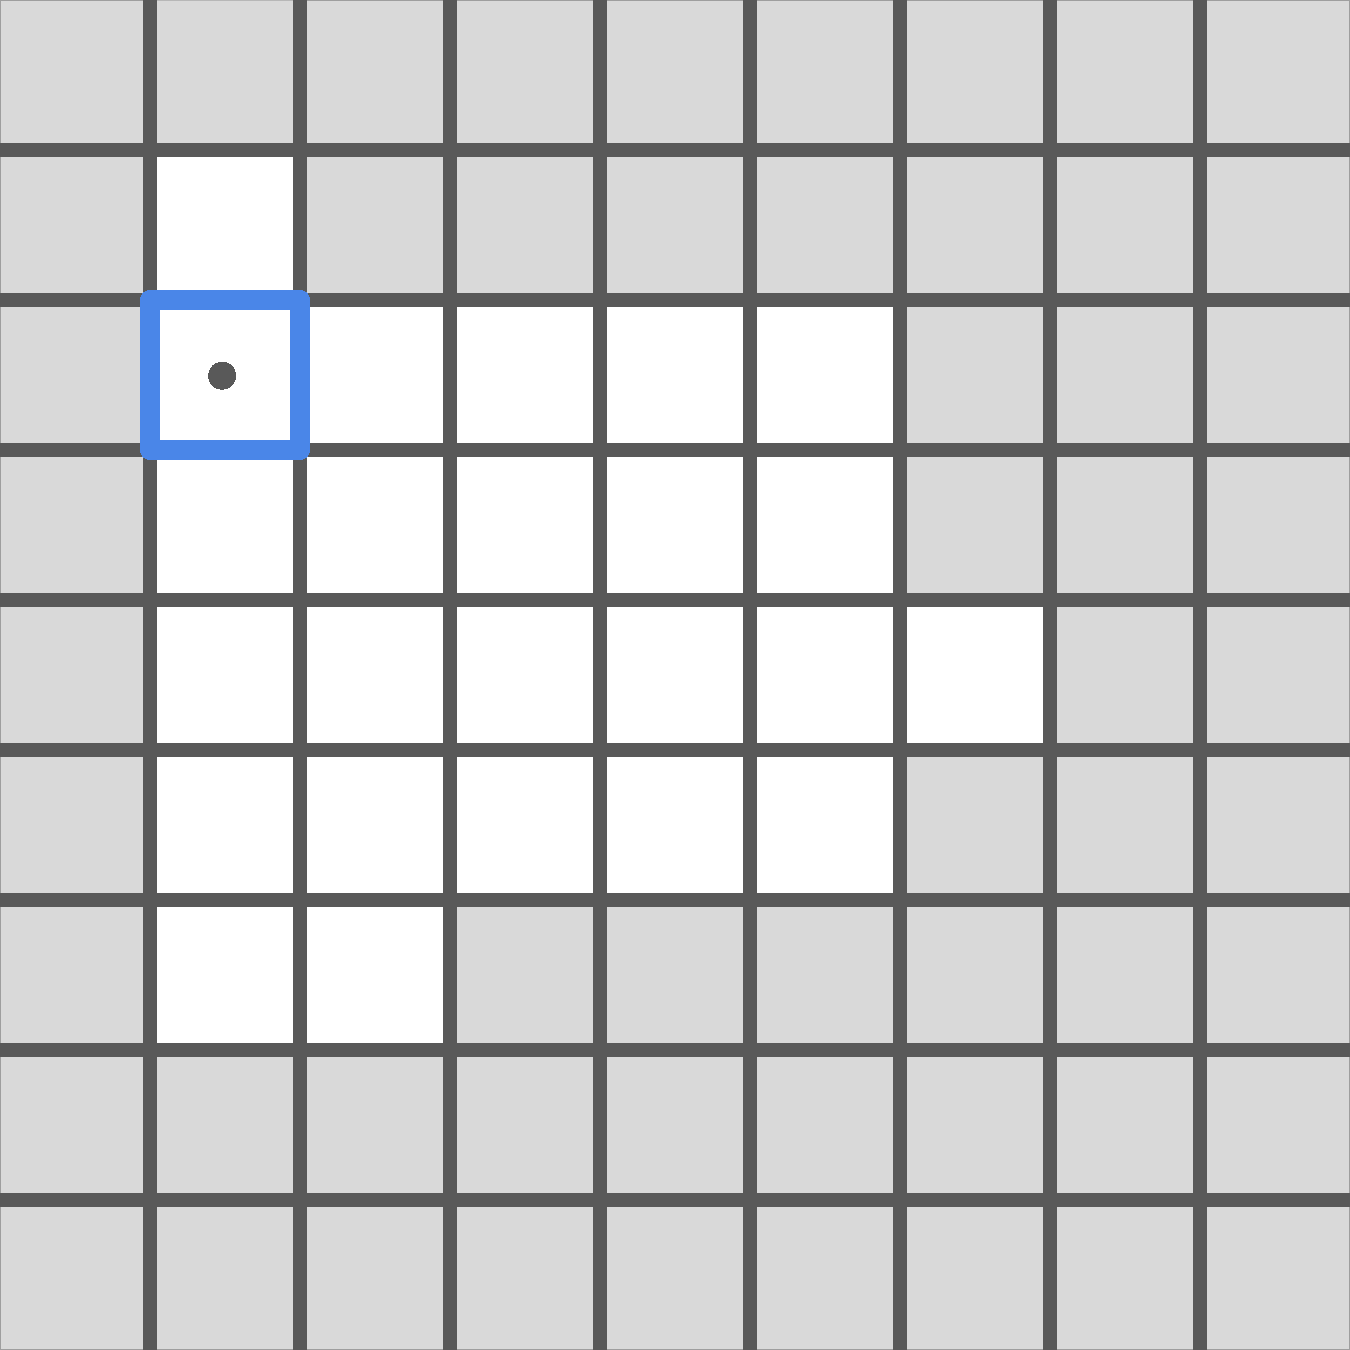
\includegraphics[width=\linewidth,trim={0 100 100 0},clip]{spiker-diagram/spiker-generate}
  \caption{cell buds developmental search prongs}
  \label{fig:budprongs}
\end{subfigure}
\begin{subfigure}[b]{0.45\linewidth}
  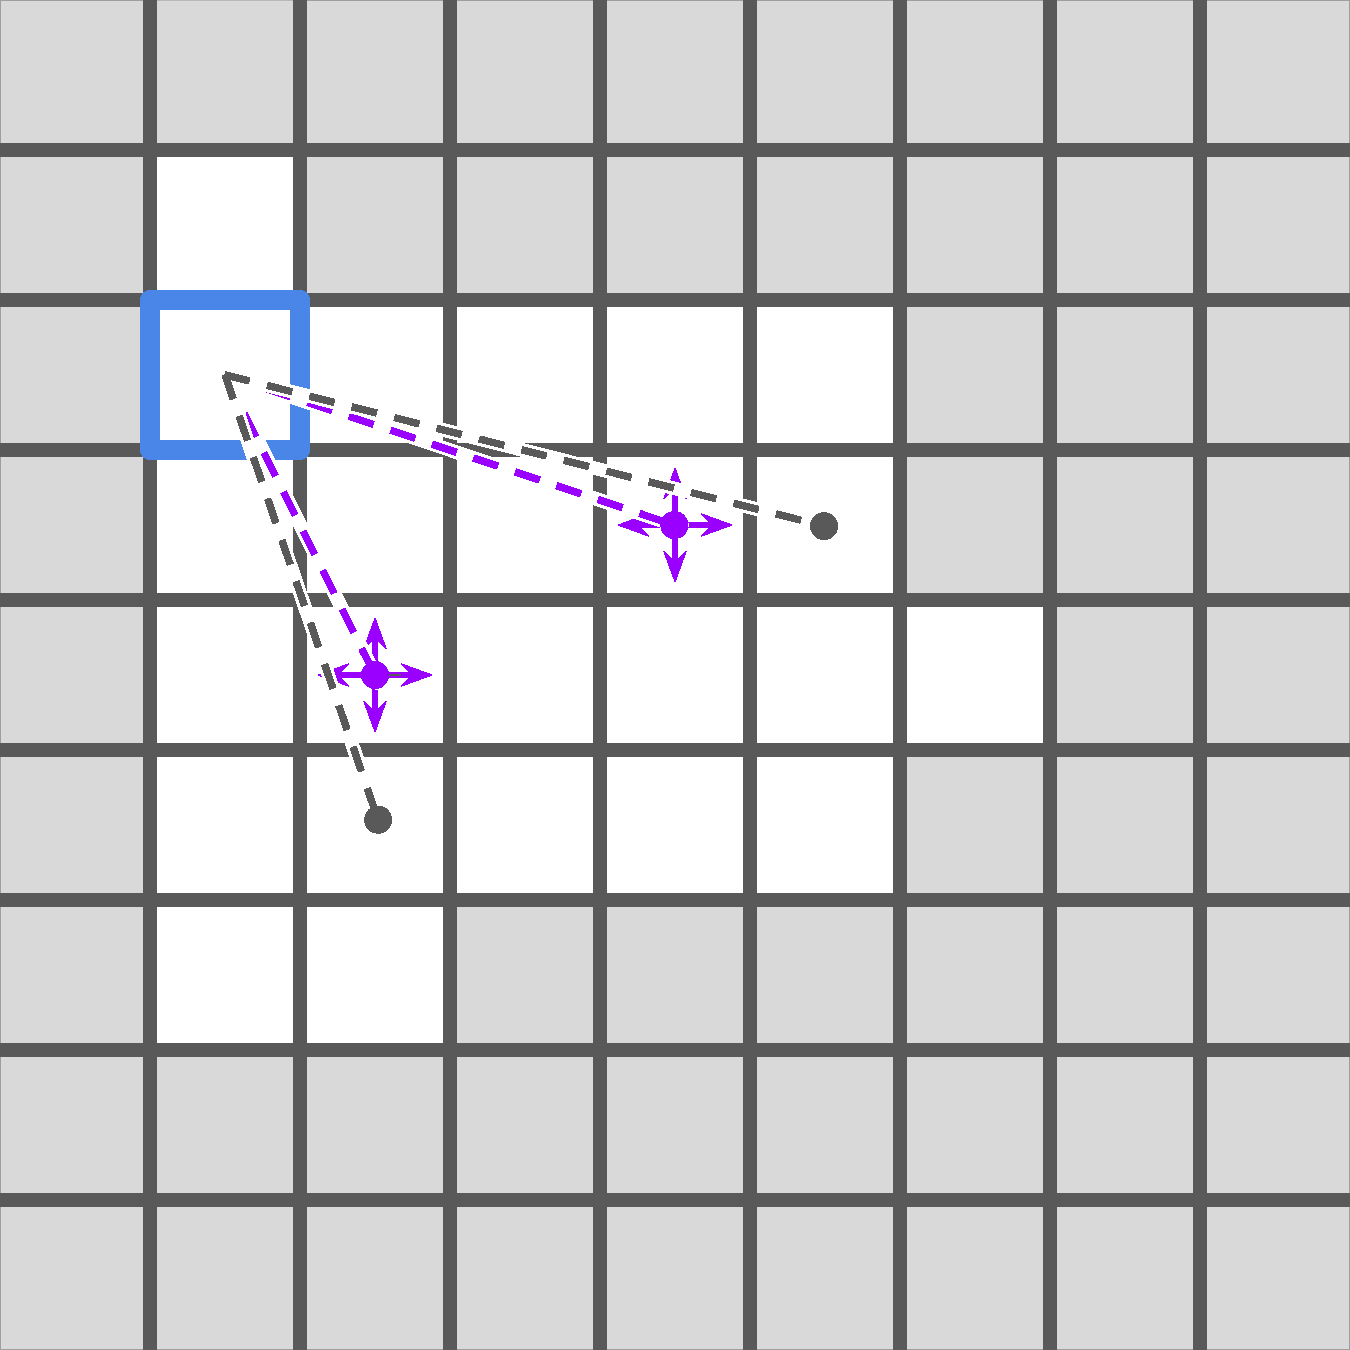
\includegraphics[width=\linewidth,trim={0 100 100 0},clip]{spiker-diagram/spiker-walk}
  \caption{search prongs perform random walk}
  \label{fig:randomwalk}
\end{subfigure}
\begin{subfigure}[b]{0.45\linewidth}
  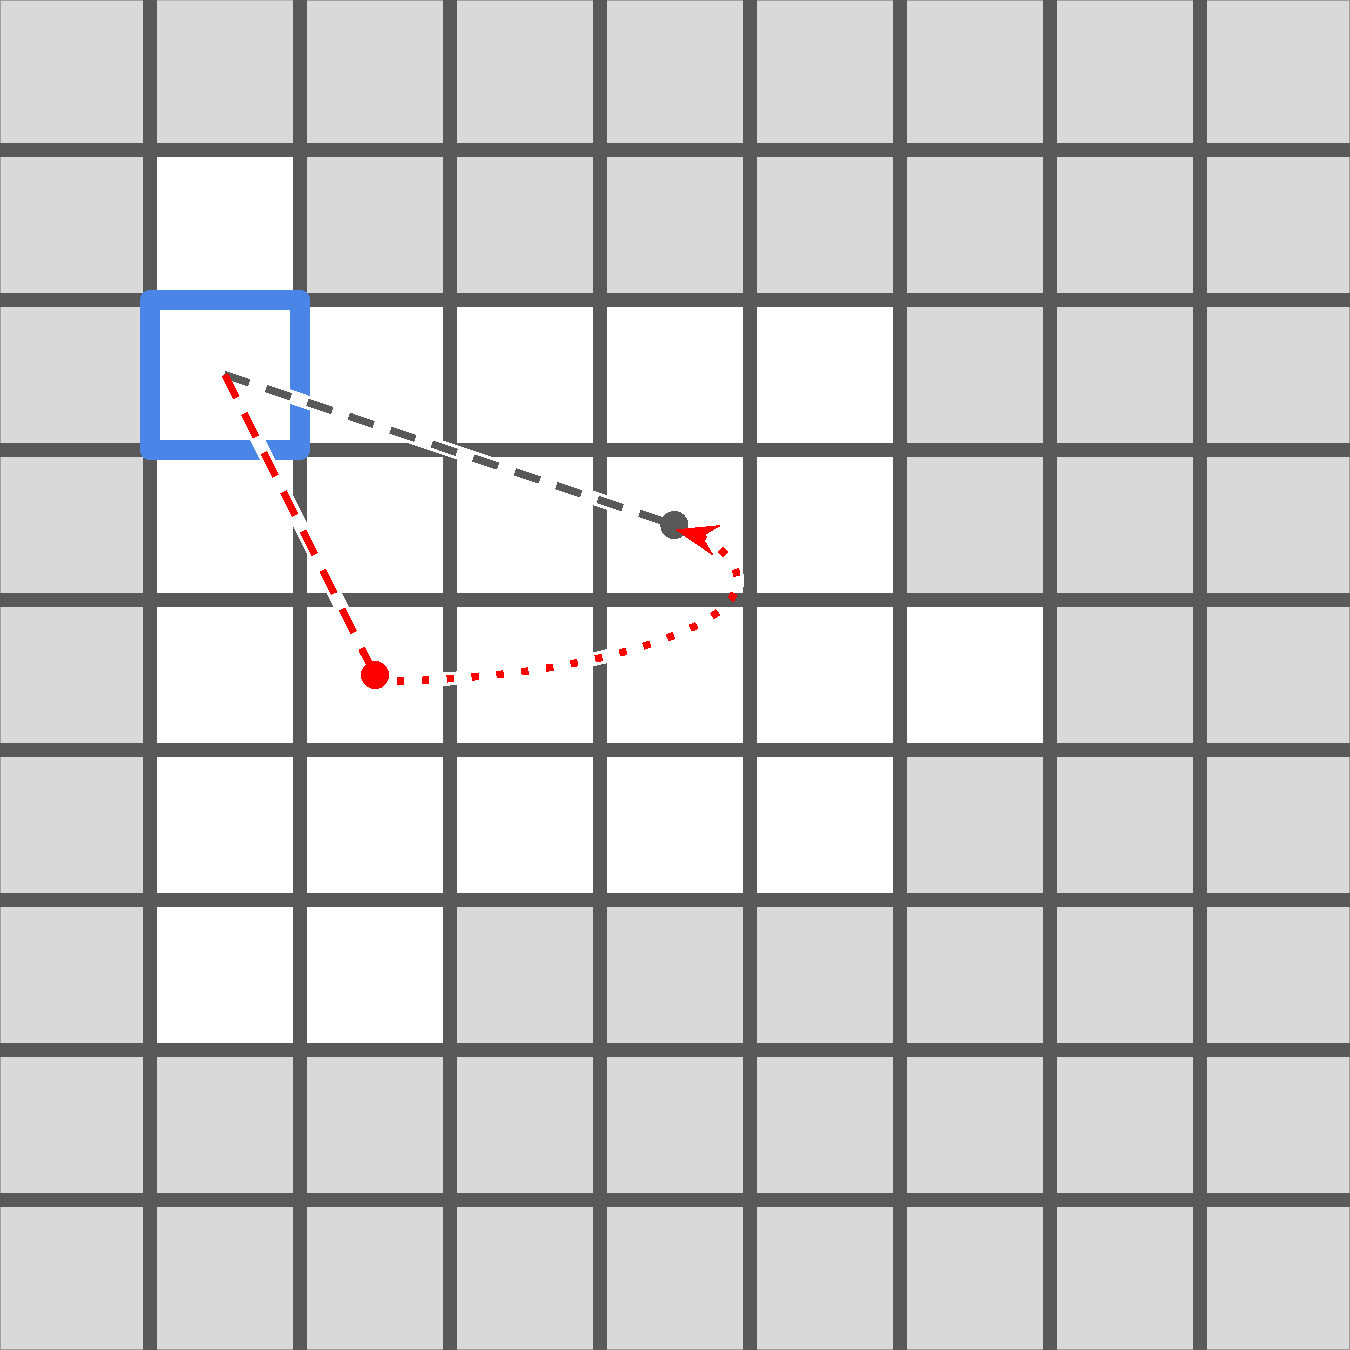
\includegraphics[width=\linewidth,trim={0 100 100 0},clip]{spiker-diagram/spiker-swap}
  \caption{poorly-performing prong resets to better-performing prong}
  \label{fig:prongreset}
\end{subfigure}
\begin{subfigure}[b]{0.45\linewidth}
  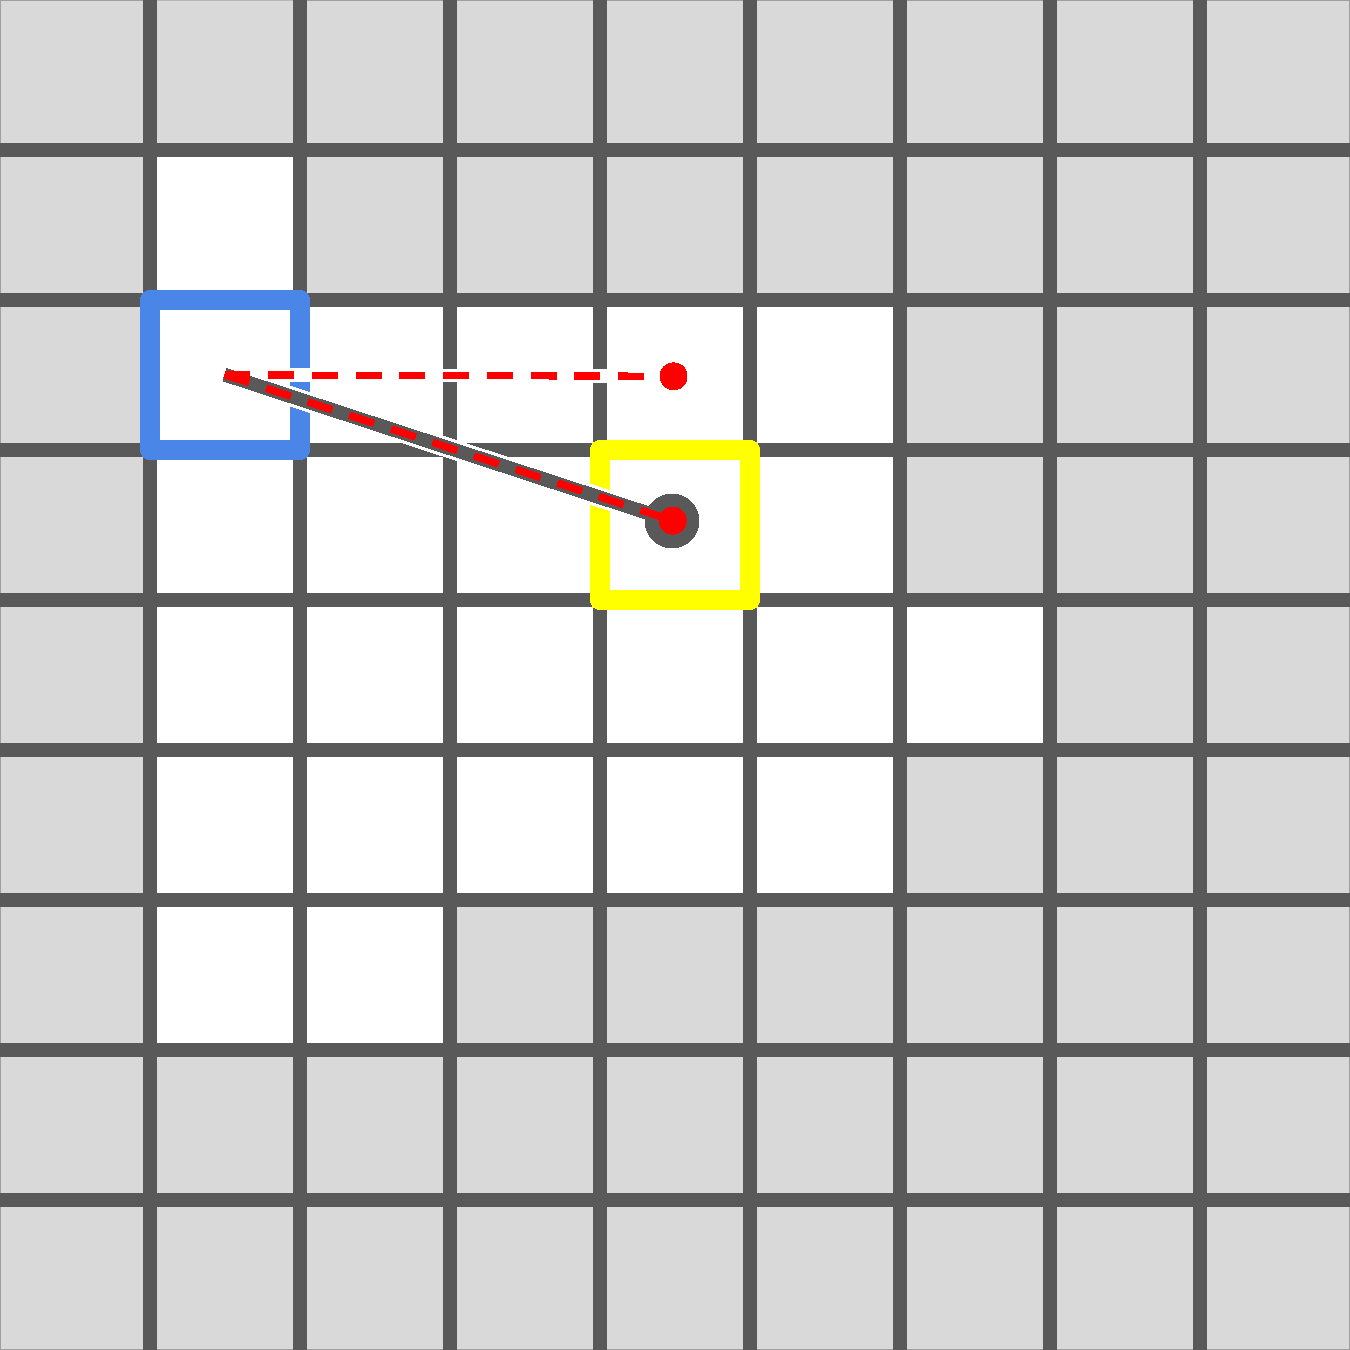
\includegraphics[width=\linewidth,trim={0 100 100 0},clip]{spiker-diagram/spiker-connect}
  \caption{search prong matures into established connection}
  \label{fig:pringmature}
\end{subfigure}
\begin{subfigure}[b]{0.45\linewidth}
  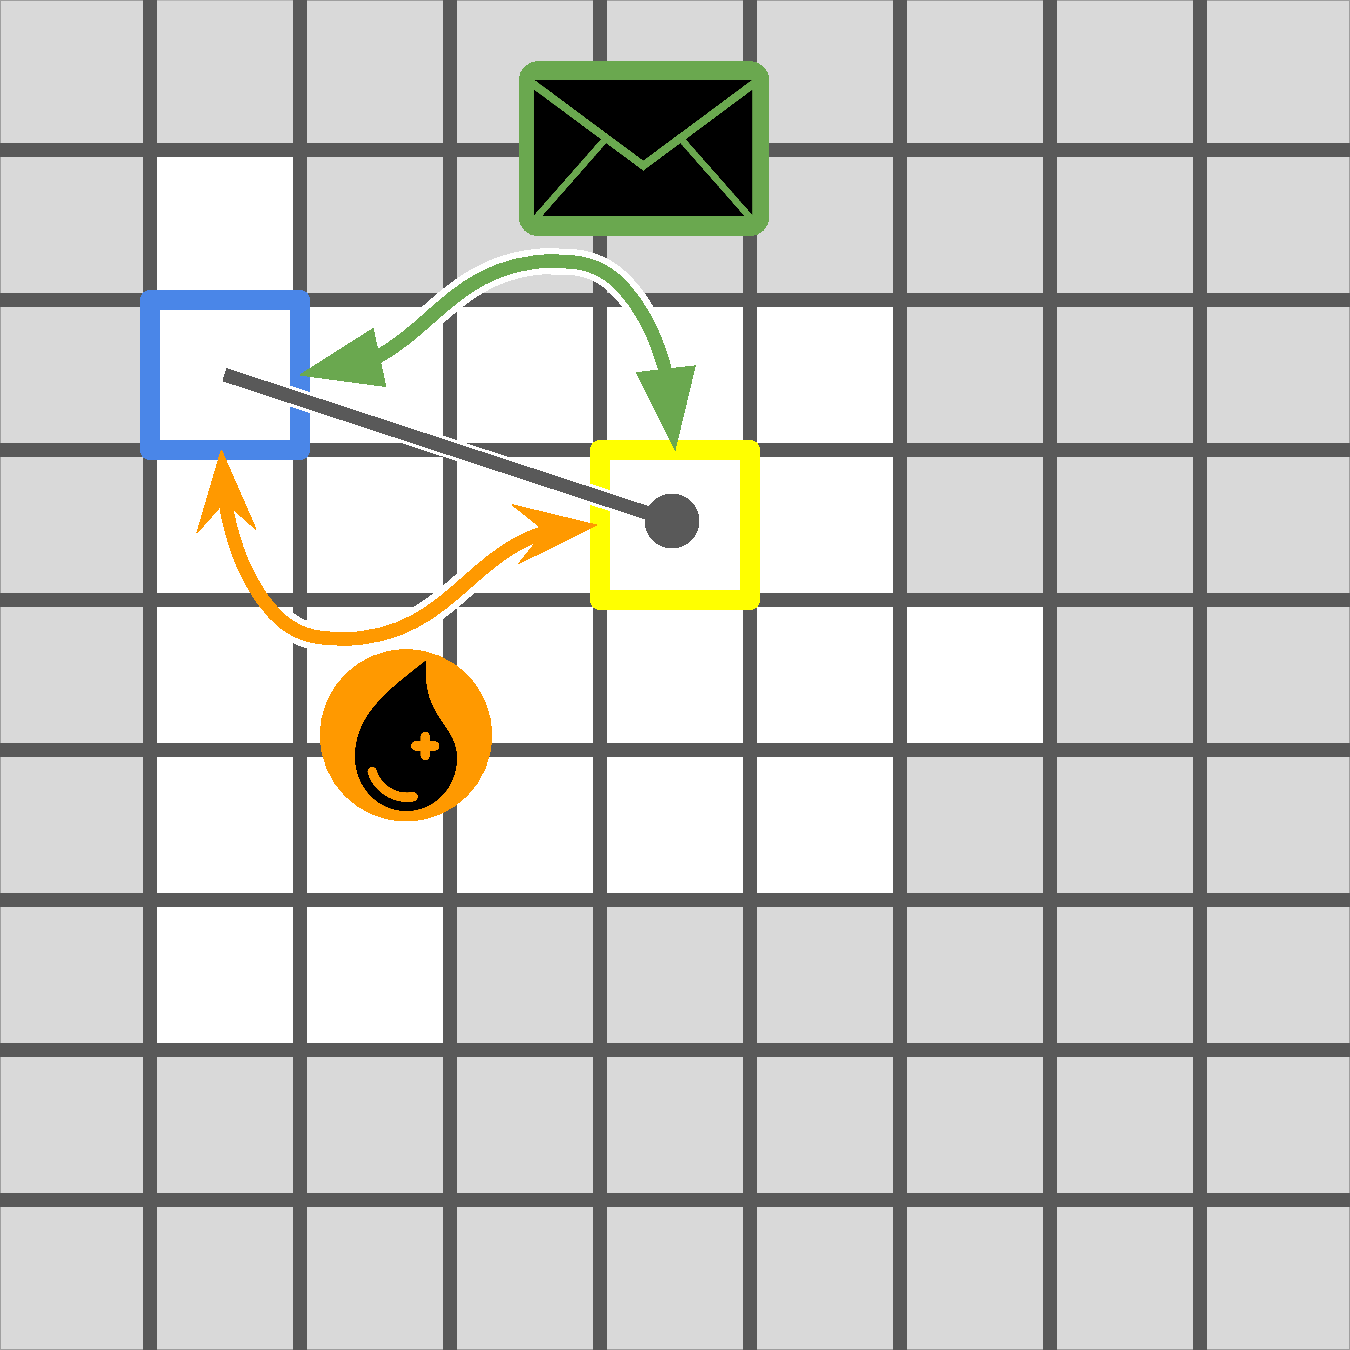
\includegraphics[width=\linewidth,trim={0 100 100 0},clip]{spiker-diagram/spiker-transmit}
  \caption{cells exchange messages over established interconnect}
  \label{fig:interconnectexchange}
\end{subfigure}
\begin{subfigure}[b]{0.45\linewidth}
  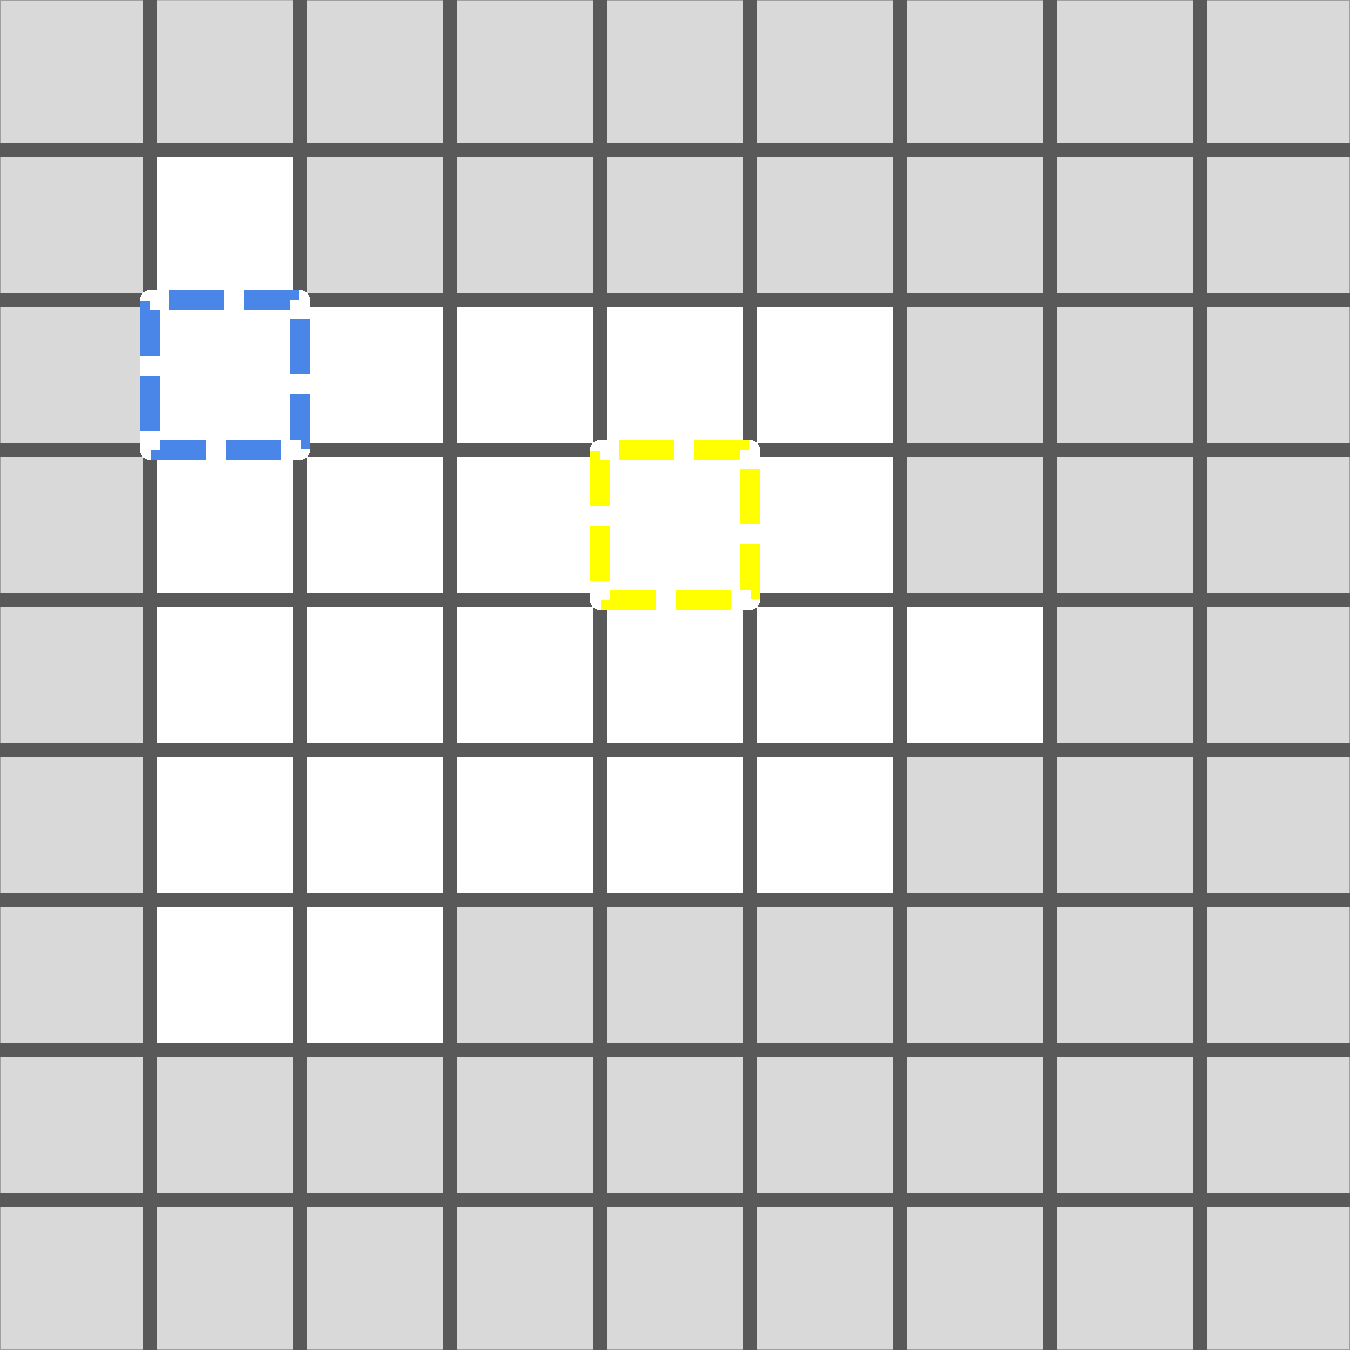
\includegraphics[width=\linewidth,trim={0 100 100 0},clip]{spiker-diagram/spiker-remove}
  \caption{established interconnects may be removed by either participating cell}
  \label{fig:interconnectremove}
\end{subfigure}
\caption{
Illustration of the developmental process used to establish long-distance interconnects.
}
\label{fig:spiker_diagram}
\end{center}
\end{figure}
